%%
%%
%%   LaTeX Beamer for ESS Presentation template
%%
%%   Jeong Han Lee, han.lee@esss.se
%%
%%   v0.1 created Monday, Monday, November 23 09:07:19 CET 2015, jhlee
%%
%%

\documentclass[
  9pt
  , table
  , ignorenonframetext
]{beamer}


\usepackage{esspre}
\usepackage{listings}

\meetingname{Timing system training for ICS integrators}
\meetingcity{Lund}
\meetingcountry{Sweden}
\totalpagenumber{\inserttotalframenumber}
%\totalpagenumber{13+}



\title{Timing system training for ICS integrators}
\author{Javier Cereijo Garcia}%\inst{1}}
\institute{
  Integrated Control System Division\\
  \textbf{ESS}, Sweden
}
\date{August 21, 2018}


\begin{document}

\begin{frame}[plain]
  \titlepage
\end{frame}


\begin{frame}{Outline}
    \begin{itemize}
    \item Timing introduction
%    \item (E3 introduction)
%    \item System configuration
%    \item e3-mrfioc2
%    \item EVR: basic start-up
%    \item EVR: basic configuration
%    \item EVR: events and triggers
%    \item EVR: timestamping
%    \item EVR: standalone mode
%    \item EVR: inputs
%    \item EVR: backplane clocks
%    \item EVG: basic start-up
%    \item EVG: basic configuration
%    \item EVG: creating events and data
    \item Data buffer
    \item Timestamping
    \item Supercycle
    \item Delay compensation
    \item SAT and SIT
    \item Deployment
    \end{itemize}
\end{frame}

\begin{frame}{Timing introduction (I...)}
  \begin{block}{Principles and requirements}
    \begin{itemize}
    \item Synchronize the operation of the facility
    \begin{itemize}
      \item Accelerator, target, neutron instruments, CF (small extent)
    \end{itemize}
    \item Provide the base frequency of 14 Hz
    \begin{itemize}
      \item Also lower (beam) repetition rates
    \end{itemize}
    \item Provide timestamping to the facility
    \begin{itemize}
      \item Data correlation, EPICS archiving
    \end{itemize}
    \item Provide trigger and clock signals
    \begin{itemize}
      \item With a defined position in an operation sequence
    \end{itemize}
    \item Support post-mortem analysis
    \begin{itemize}
      \item What was the cause of a beam trip?
    \end{itemize}
    \end{itemize}
  \end{block}
\end{frame}

\begin{frame}{Timing introduction (...II...)}
  \begin{block}{Implementation principles}
    \begin{itemize}
    \item A single master unit controls the timing distribution
    \begin{itemize}
      \item Control from one central point
    \end{itemize}
    \item Client units (receivers) act on master’s orders
    \begin{itemize}
      \item No dependency on e.g. computer network traffic
      \item Actions pre-programmed at the receivers
    \end{itemize}
    \item Synchronization to RF
    \begin{itemize}
      \item All timing clocks phase-synchronous to RF (subharmonic)
    \end{itemize}
    \item Distributes "wall-clock" time from the master
      \item Timestamp support in hardware
    \begin{itemize}
      \item Used for data reconstruction and correlation
    \end{itemize}
    \end{itemize}
  \end{block}
\end{frame}

\begin{frame}{Timing introduction (...III...)}
  \begin{columns}
    \begin{column}{.6\textwidth}
      \begin{block}{Structure of the system}
        \begin{itemize}
          \item Master Event Generator (EVG) generates a continuous data stream
          \item The (accelerator) synchronization frequency (of 88 MHz) will be fed into the master event generator and used as the system clock. Event receivers synchronize to that clock.
          \item The 14 Hz operating frequency will be generated by down conversion from RF in the event generator (divide 88.0525 MHz by 6289464 to get 14.00000064 Hz)
          \item All timing sequences, events, etc., generated in hardware
          \item Links work upstream, too
        \end{itemize}
      \end{block}
    \end{column}
    \begin{column}{.5\textwidth}
      \centering
      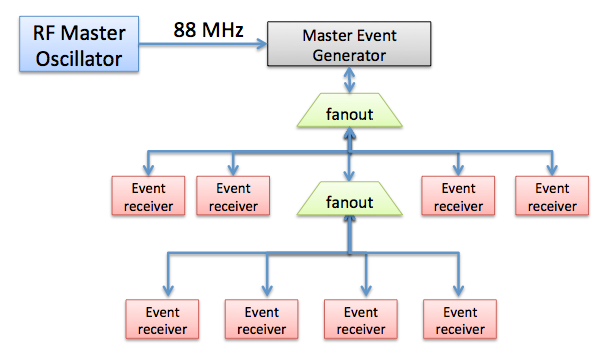
\includegraphics[width=1\textwidth]{./pictures/TimingDistribution.png}
    \end{column}
  \end{columns}
\end{frame}

\begin{frame}{Timing introduction (...IV...)}
  \begin{block}{On-the-wire protocol}
    \centering
    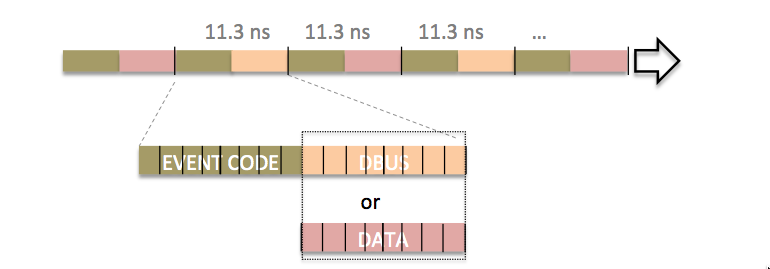
\includegraphics[width=0.6\textwidth]{./pictures/BitStream.png}
    \begin{itemize}
      \item 16-bit "frame" repeating at 88.0525 MHz (11.3 ns), i.e. 352.2 MHz/4
      \item Each frame contains an 8-bit event code and alternating distributed bus/data byte (8 bits).
      \item Distributed bus (DBus) broadcasts eight binary signals which can be output from each Event Receiver. Clocks, status bits, etc.
      \item Event Generator can broadcast arbitrary data (up to 2kB blocks)
      \item Data buffer sent one byte at a time and collected at the receiver(s)
      \item Trigger events and DBUS/Data are independent of each other
    \end{itemize}
  \end{block}
\end{frame}

\begin{frame}{Timing introduction (...V...)}
  \begin{block}{Events, clocks and data}
    \begin{itemize}
      \item Meaning of "event" in this context: signal at a precise time
      \begin{itemize}
        \item Hardware outputs with programmable delay, width, polarity
        \item Event can also trigger software (EPICS) to do actions
        \begin{itemize}
          \item "Collect post-mortem data now", "start counting", etc.
        \end{itemize}
        \item Events can be (synchronously) time-stamped
        \item "Upstream" events: from EVR to EVG (and back)
      \end{itemize}
      \item Clock: a repetitive sequence of pulses
      \begin{itemize}
        \item E.g., a 1 kHz synchronization clock
      \end{itemize}
      \item Data transmission
      \begin{itemize}
        \item Limited amount of data delivered synchronously
        \item For configuration and validation purposes
        \item Still under development (some space for requests)
      \end{itemize}
    \end{itemize}
  \end{block}
\end{frame}

\begin{frame}{Timing introduction (...VI...)}
  \begin{block}{Accelerator cycle}
    \centering
    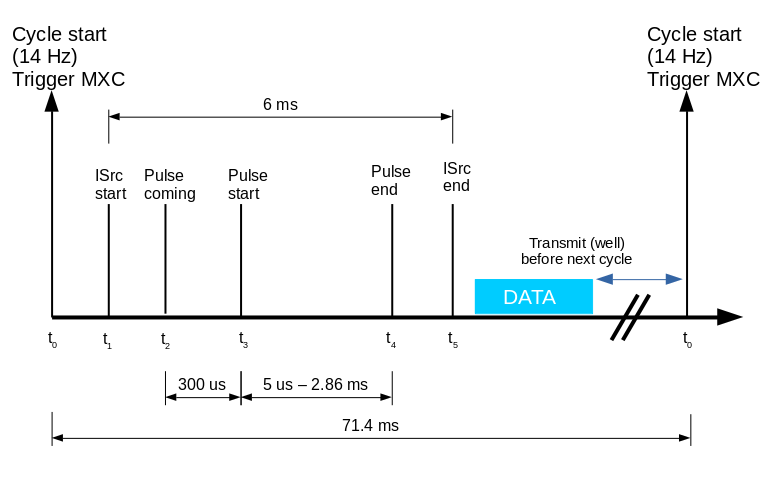
\includegraphics[width=0.5\textwidth]{./pictures/AccCycle.png}
    \begin{itemize}
      \item Pre-programmed sequences repeat at 14 Hz
      \begin{itemize}
        \item Hardware-based (FPGA) sequencer with a RF-synchronous 88 MHz clock
        \item "Programming" can happen in less than a millisecond
      \end{itemize}
      \item "Data", i.e., beam mode, etc., transmitted in parallel
      \begin{itemize}
        \item Contains "plan" for the next cycle: envelope mode, beam/no beam, pulse counter, rep rate, ...
        \item Mode changes require a handshake with BIS
        \begin{itemize}
          \item When mode change is transmitted, timing does not send beam before MPS/BIS gives OK
        \end{itemize}
      \end{itemize}
    \end{itemize}
  \end{block}
\end{frame}

\begin{frame}{Timing introduction (...VII...)}
  \begin{block}{Timing adjustment policy}
    \begin{itemize}
      \item Local delay settings are used for local fine-tuning; adjusting for propagation, processing, etc., delays during commissioning
      \item Pulse length, etc. information in beam data buffer is not for setting the pulse timing locally but for:
      \begin{itemize}
        \item Pulse verification, feed-back/forward, etc.
      \end{itemize}
      \item ”Beam off” will be a dedicated event. A ”gate” signal will be set on with a ”beam on” event and set off with a ”beam off” event
      \begin{itemize}
        \item Central handling of the beam duration, no software activity needed at the (hundreds of ) local receivers (to set the delays)
        \item Actions can be tied to the beam off event, like beam-sync data collection and broadcast
        \item Pulse may be cut short by the timing system. Separate event will allow clean handling of the early pulse abort
      \end{itemize}
    \end{itemize}
  \end{block}
\end{frame}

\begin{frame}{Timing introduction (... and VIII)}
  \begin{block}{Documentation}
    \begin{itemize}
      \item ESS Timing System System Architecture Description - ESS-0088633
      \item Data Model Specification for the ESS Timing System - ESS-0225673
      \item Event System with Delay Compensation Technical Reference - \url{http://mrf.fi/}
      \item EVR Usage Guide - \url{http://epics.sourceforge.net/mrfioc2/evr-usage.pdf} or \url{https://github.com/epics-modules/mrfioc2/blob/master/documentation/evr-usage.lyx} (lyx version)
      \item Manuals in CHESS
    \end{itemize}
  \end{block}
\end{frame}

%\begin{frame}[fragile]{(E3 introduction (I...))}
%\begin{lstlisting}[style=termstyle,breaklines=true,basicstyle=\scriptsize]
%[iocuser@icslab-ts03 ics_gitsrc]$ git clone https://github.com/icshwi/e3
%
%[iocuser@icslab-ts03 e3-mrfioc2]$ ./e3.bash -t all
%
%[iocuser@icslab-ts03 ~]$ source ~/ics_gitsrc/e3/tools/setenv
%
%Set the ESS EPICS Environment as follows:
%THIS Source NAME    : setE3Env.bash
%THIS Source PATH    : /epics/base-3.15.5/require/3.0.0/bin
%EPICS_BASE          : /epics/base-3.15.5
%EPICS_HOST_ARCH     : linux-x86_64
%E3_REQUIRE_LOCATION : /epics/base-3.15.5/require/3.0.0
%PATH                : /epics/base-3.15.5/require/3.0.0/bin:/epics/base-3.15.5/bin/linux-x86_64:/usr/local/bin:/usr/bin:/usr/local/sbin:/usr/sbin:/home/iocuser/.local/bin:/home/iocuser/bin
%LD_LIBRARY_PATH     : /epics/base-3.15.5/lib/linux-x86_64:/epics/base-3.15.5/require/3.0.0/lib/linux-x86_64:/epics/base-3.15.5/require/3.0.0/siteLibs/linux-x86_64
%
%Enjoy E3!
%\end{lstlisting}
%\end{frame}
%
%\begin{frame}[fragile]{(E3 introduction (... and II))}
%\begin{lstlisting}[style=termstyle,breaklines=true,basicstyle=\footnotesize]
%[iocuser@icslab-ts03 ics_gitsrc]$ git clone https://github.com/icshwi/essics_scripts
%
%[iocuser@icslab-ts03 ics_gitsrc]$ bash essics_scripts/iocuser_env/iocuser_env_setup.bash clean
%
%[iocuser@icslab-ts03 ics_gitsrc]$ bash  essics_scripts/iocuser_env/iocuser_env_setup.bash install
%
%[iocuser@icslab-ts03 ics_gitsrc]$ bash  essics_scripts/iocuser_env/iocuser_env_setup.bash link
%
%\end{lstlisting}
%\end{frame}

%\begin{frame}[fragile]{System configuration (I...)}
%\begin{lstlisting}[style=termstyle,breaklines=true,basicstyle=\scriptsize]
%[iocuser@icslab-ts03 ~]$ lspci
%0a:00.0 Signal processing controller: Xilinx Corporation Device 7011
%[iocuser@icslab-ts03 ~]$ lspci -s a:0 -vv
%0a:00.0 Signal processing controller: Xilinx Corporation Device 7011
%	Subsystem: Device 1a3e:132c
%	Physical Slot: 1-1
%	Control: I/O+ Mem+ BusMaster+ SpecCycle- MemWINV- VGASnoop- ParErr- Stepping- SERR- FastB2B- DisINTx-
%	Status: Cap+ 66MHz- UDF- FastB2B- ParErr- DEVSEL=fast >TAbort- <TAbort- <MAbort- >SERR- <PERR- INTx-
%	Latency: 0, Cache Line Size: 64 bytes
%	Interrupt: pin A routed to IRQ 7
%	Region 0: Memory at c0600000 (32-bit, non-prefetchable) [size=256K]
%	Capabilities: <access denied>
%
%\end{lstlisting}
%\end{frame}
%
%\begin{frame}[fragile]{System configuration (...II...)}
%\begin{lstlisting}[style=termstyle,breaklines=true,basicstyle=\scriptsize]
%[iocuser@icslab-ts03 ics_gitsrc]$ git clone https://github.com/jeonghanlee/pciids
%
%[iocuser@icslab-ts03 pciids]$ sh replace-pciids.bash
%
%[iocuser@icslab-ts03 pciids]$ lspci -s a:0 -vv
%0a:00.0 Signal processing controller: Xilinx Corporation XILINX PCI DEVICE
%	Subsystem: Micro-Research Finland Oy MTCA Event Receiver 300
%	Physical Slot: 1-1
%	Control: I/O+ Mem+ BusMaster+ SpecCycle- MemWINV- VGASnoop- ParErr- Stepping- SERR- FastB2B- DisINTx-
%	Status: Cap+ 66MHz- UDF- FastB2B- ParErr- DEVSEL=fast >TAbort- <TAbort- <MAbort- >SERR- <PERR- INTx-
%	Latency: 0, Cache Line Size: 64 bytes
%	Interrupt: pin A routed to IRQ 7
%	Region 0: Memory at c0600000 (32-bit, non-prefetchable) [size=256K]
%	Capabilities: <access denied>
%
%\end{lstlisting}
%\end{frame}
%
%\begin{frame}[fragile]{System configuration (...III...)}
%\begin{lstlisting}[style=termstyle,breaklines=true,basicstyle=\footnotesize]
%[iocuser@icslab-ts03 e3-mrfioc2]$ make init
%
%[iocuser@icslab-ts03 e3-mrfioc2]$ make dkms_add
%
%[iocuser@icslab-ts03 e3-mrfioc2]$ make dkms_build
%
%[iocuser@icslab-ts03 e3-mrfioc2]$ make dkms_install
%
%[iocuser@icslab-ts03 e3-mrfioc2]$ make setup
%
%\end{lstlisting}
%\end{frame}
%
%\begin{frame}[fragile]{System configuration (... and IV)}
%\begin{lstlisting}[style=termstyle,breaklines=true,basicstyle=\scriptsize]
%[iocuser@icslab-ts03 e3-mrfioc2]$ systemctl status dkms
%● dkms.service - Builds and install new kernel modules through DKMS
%   Loaded: loaded (/usr/lib/systemd/system/dkms.service; enabled; vendor preset: enabled)
%   Active: active (exited) since Fri 2018-08-17 10:28:19 CEST; 57s ago
%     Docs: man:dkms(8)
%  Process: 793 ExecStart=/bin/sh -c dkms autoinstall --verbose --kernelver $(uname -r) (code=exited, status=0/SUCCESS)
% Main PID: 793 (code=exited, status=0/SUCCESS)
%    Tasks: 0
%   CGroup: /system.slice/dkms.service
%
%Aug 17 10:28:18 icslab-ts03 systemd[1]: Starting Builds and install new kernel modules through DKMS...
%Aug 17 10:28:19 icslab-ts03 systemd[1]: Started Builds and install new kernel modules through DKMS.
%\end{lstlisting}
%\end{frame}

%\begin{frame}{e3-mrfioc2}
%  \begin{itemize}
%    \item \url{https://github.com/icshwi/e3-mrfioc2/}
%    \item Cmds: startup scripts
%    \item Opi: community opis with ESS naming (check readme for opis up to date)
%    \item Template: substitutions files
%    \item Installation path: /epics/base-3.15.5/require/3.0.0/siteMods/mrfioc2/2.2.0-rc2/db/
%  \end{itemize}
%\end{frame}

\begin{frame}{Data buffer}
  \begin{block}{Data buffer}
    \url{https://confluence.esss.lu.se/display/HAR/Data+Buffer}
    \url{https://confluence.esss.lu.se/display/HAR/Event+and+Trigger+Reference}
    \begin{itemize}
      \item Protocol number
      \item Protocol version
      \item Linac cycle counter/ID & Heartbeat
      \item Proton beam status
      \item Proton beam destination (last point)
      \item Proton beam mode
      \item Proton beam present
      \item Proton beam length
      \item Proton beam energy
      \item Proton beam current
      \item Raster pattern
      \item Target segment
\end{itemize}
  \end{block}
\end{frame}

\begin{frame}[fragile]{Timestamping}
\url{https://github.com/icshwi/esstex/tree/master/document/ics_eng_docs_timestamping}
\begin{lstlisting}[style=termstyle,breaklines=true,basicstyle=\scriptsize]

6690f8a.icslab-ipc01.14335 > generalTimeReport
Backwards time errors prevented 0 times.

Current Time Providers:
    "EVR", priority = 50
        Current Time is 2018-08-13 11:18:40.234652.
    "OS Clock", priority = 999
        Current Time is 2018-08-13 11:20:05.683007.

Event Time Providers:
    "EVR", priority = 50

\end{lstlisting}
\end{frame}

\begin{frame}{Supercycle (I...)}
  \begin{block}{Supercycle}
    \begin{itemize}
      \item Supercycle: a predefined sequence of machine cycles:
      \begin{itemize}
        \item Timing pattern
        \item Beam parameter (data)
      \end{itemize}
      \item Cycles are pre-configured (with a control-room application)
      \item E.g., a supercycle for:
      \begin{itemize}
        \item 1 Hz operation must have 1 cycle with beam, 13 cycles without beam
        \item 0.1 Hz: 1 cycle with beam,  139 cycles without beam
      \end{itemize}
      \item Editor application allows to define
      \begin{itemize}
        \item pulse length (timing events in HW sequencer)
        \item beam current (iris change, probably not between cycles)
        \item pulse delay (within 2.86 time window, in sequencer)
        \item beam destination (in data buffer)
        \item beam mode (in data buffer)
        \item etc.
      \end{itemize}
    \end{itemize}
  \end{block}
\end{frame}

\begin{frame}[fragile]{Supercycle (... and II)}
  \begin{block}{Example}
    \begin{itemize}
      \item Example from \url{https://gitlab.esss.lu.se/icshwi/reftabs/-/blob/master/supercycles/example-noCalib-2Hz-14c.csv}.
    \end{itemize}
    \begin{lstlisting}[style=termstyle,breaklines=true,basicstyle=\scriptsize]
Id,IonMagSt,IonMagEnd,RFSt,LEBTCSt,LEBTCEnd,MEBTCSt,MEBTCEnd,BPulseSt,BPulseEnd,BLen,BEn,BCurr
0,10000,10050,10010,10100,10150,10200,10250,13300,13350,50,100,100000
1,,,10011,10100,10151,10200,10251,13300,13350,51,101,100001
2,,,10012,10100,10152,10200,10252,13300,13350,52,102,100002
3,,,10013,10100,10153,10200,10253,13300,13350,53,103,100003
4,,,10014,10100,10154,10200,10254,13300,13350,54,104,100004
5,,,10015,10100,10155,10200,10255,13300,13350,55,105,100005
6,,,10016,10100,10156,10200,10256,13300,13350,56,106,100006
7,10000,10060,10017,10100,10157,10200,10257,13300,13350,57,107,100007
8,,,10018,10100,10158,10200,10258,13300,13350,58,108,100008
9,,,10019,10100,10159,10200,10259,13300,13350,59,109,100009
10,,,10020,10100,10160,10200,10260,13300,13350,60,110,100010
11,,,10021,10100,10161,10200,10261,13300,13350,61,111,100011
12,,,10022,10100,10162,10200,10262,13300,13350,62,112,100012
13,,,10023,10100,10163,10200,10263,13300,13350,63,113,100013

    \end{lstlisting}
  \end{block}
\end{frame}

\begin{frame}{Delay compensation}
  \begin{block}{DC}
    Delay compensation is achieved in measuring the propagation delay of events from the delay compensation master EVM through the distribution network up to the Event Receivers. At the last stage the EVR is aware of the delay through the network and adjusts an internal FIFO depth to match a programmed target delay value.
  \end{block}
\end{frame}

\begin{frame}{SAT and SIT}
  \begin{block}{SAT and SIT}
    \begin{itemize}
      \item When EVR is installed in FEB/G02: SAT and SIT.
      \item Jerzy does it.
      \item \url{https://confluence.esss.lu.se/display/HAR/Acceptance}
      \item SAT: check that the HW is OK, MCH correctly configured, fibres in place, etc.
      \item SIT: check that the EVR is working fine, receives events from the EVG, correctly creates trigger and gate signals, etc.
    \end{itemize}
  \end{block}
\end{frame}

\begin{frame}[fragile]{Deployment}
  \begin{block}{Deployment}
    \begin{lstlisting}[style=termstyle,breaklines=true,basicstyle=\scriptsize]
require "autosave" "5.10.2"
require "mrfioc2" "2.3.1-beta.3.3"
epicsEnvSet "PEVR" "SYS-SUB:Ctrl-EVR-101"
epicsEnvSet "PCI_SLOT" "08:00.0"
epicsEnvSet "OUTARGS" "WIDTH0=1000, EVT0T0=14, BP0SRC=0, WIDTH1=1000, EVT1T0=15, BP1SRC=1, WIDTH2=10, EVT2T0=12, WIDTH3=10, EVT3T0=13, BP2SRC=49, WIDTH4=1000, EVT4T0=125, BP3SRC=4, WIDTH5=1000,  EVT5T0=40, BP4SRC=5, WIDTH7=1000, EVT7T0=42, BP6SRC=7,"
epicsEnvSet "INARGS" "BPIN5=, BP5EVT=41, BPIN7=, BP7EVT=43,"

    \end{lstlisting}
  \end{block}
\end{frame}

\begin{frame}{Questions?}
  \begin{center}
    {\Huge Questions?}
  \end{center}
\end{frame}

\begin{frame}[fragile]{EVR: basic start-up}
\begin{lstlisting}[style=termstyle,breaklines=true,basicstyle=\scriptsize]
### Load the mrfioc2 module ###
require mrfioc2,2.2.0-rc2

### Define several needed macros ###
epicsEnvSet("IOC", "TRAINING")
epicsEnvSet("DEV1", "EVR1")
epicsEnvSet("MainEvtCODE" "14")
epicsEnvSet("HeartBeatEvtCODE"   "122")
epicsEnvSet("ESSEvtClockRate"  "88.0525")

### Register the EVR with the IOC and load the database ###
mrmEvrSetupPCI("$(DEV1)",  "0a:00.0")
dbLoadRecords("evr-mtca-300u-ess.db","EVR=$(DEV1), SYS=$(IOC), D=$(DEV1), FEVT=$(ESSEvtClockRate)")

### Needed with software timestamp source w/o RT thread scheduling ###
var evrMrmTimeNSOverflowThreshold 100000


iocInit()

### Set delay compensation to 70 ns, needed to avoid timesptamp issue ###
dbpf $(IOC)-$(DEV1):DC-Tgt-SP 70

\end{lstlisting}
\end{frame}

\begin{frame}[fragile]{EVR: basic configuration}
\begin{lstlisting}[style=termstyle,breaklines=true,basicstyle=\scriptsize]
[iocuser@icslab-ts03 cmds]$ iocsh.bash TRAINING-EVR1.cmd

caget TRAINING-EVR1:Link-Sts
caget TRAINING-EVR1:Link-Clk-I
caget TRAINING-EVR1:Cnt-LinkTimo-I
caput TRAINING-EVR1:Link-Clk-SP 100
caget TRAINING-EVR1:Link-Clk-I
caget TRAINING-EVR1:Link-Sts
caget TRAINING-EVR1:Cnt-LinkTimo-I
caget TRAINING-EVR1:Cnt-LinkTimo-I
caput TRAINING-EVR1:Link-Clk-SP 88.0525
caget TRAINING-EVR1:Link-Clk-I
caget TRAINING-EVR1:Link-Sts

caget TRAINING-EVR1:Time-Valid-Sts

caget TRAINING-EVR1:FwVer-I

\end{lstlisting}
\end{frame}

\begin{frame}[fragile]{EVR: events and triggers}
\begin{lstlisting}[style=termstyle,breaklines=true,basicstyle=\scriptsize]
camonitor TRAINING-EVR1:EvtECnt-I

caput TRAINING-EVR1:DlyGen0-Evt-Trig0-SP 14

caput TRAINING-EVR1:DlyGen0-Width-SP 1000

caput TRAINING-EVR1:OutFP0-Src-SP 0

/epics/base-3.15.5/require/3.0.0/siteMods/mrfioc2/2.2.0-rc2/db/evr-mtca-300u-ess.db

TRAINING-EVR1:OutFP0-Src-Pulse-SP
TRAINING-EVR1:OutFP0-Src-DBus-SP
TRAINING-EVR1:OutFP0-Src-Scale-SP

\end{lstlisting}
\end{frame}

\begin{frame}[fragile]{EVR: timestamping}
\url{https://github.com/icshwi/esstex/tree/master/document/ics_eng_docs_timestamping}
\begin{lstlisting}[style=termstyle,breaklines=true,basicstyle=\scriptsize]

6690f8a.icslab-ipc01.14335 > generalTimeReport
Backwards time errors prevented 1464 times.

Current Time Providers:
    "EVR", priority = 50
        Current Time is 2018-08-13 11:18:40.234652.
    "OS Clock", priority = 999
        Current Time is 2018-08-13 11:20:05.683007.

Event Time Providers:
    "EVR", priority = 50


dbLoadRecords("./counter.db")

camonitor counter

caput TRAINING-EVR1:Time-I.EVNT 14
caput TRAINING-EVR1:Time-I.INP "@OBJ=EVR1, Code=14"
caput counter.TSEL TRAINING-EVR1:Time-I.TIME

\end{lstlisting}
\end{frame}

\begin{frame}[fragile]{EVR: standalone mode (I...)}
\begin{lstlisting}[style=termstyle,breaklines=true,basicstyle=\scriptsize]
### Load the mrfioc2 module ###
require mrfioc2,2.2.0-rc2

### Define several needed macros ###
epicsEnvSet("IOC", "TRAINING")
epicsEnvSet("DEV1", "EVR1")
epicsEnvSet("MainEvtCODE" "14")
epicsEnvSet("HeartBeatEvtCODE"   "122")
epicsEnvSet("ESSEvtClockRate"  "88.0525")

### Register the EVR with the IOC and load the database ###
mrmEvrSetupPCI("$(DEV1)",  "0a:00.0")
dbLoadRecords("evr-mtca-300u-ess.db","EVR=$(DEV1), SYS=$(IOC), D=$(DEV1), FEVT=$(ESSEvtClockRate)")

### Needed with software timestamp source w/o RT thread scheduling ###
var evrMrmTimeNSOverflowThreshold 100000

\end{lstlisting}
\end{frame}

\begin{frame}[fragile]{EVR: standalone mode (...II...)}
\begin{lstlisting}[style=termstyle,breaklines=true,basicstyle=\scriptsize]
iocInit()

### Set delay compensation to 70 ns, needed to avoid timesptamp issue ###
dbpf $(IOC)-$(DEV1):DC-Tgt-SP 70

### Get current time from system clock ###
dbpf $(IOC)-$(DEV1):TimeSrc-Sel "Sys. Clock"

### Set up the prescaler that will trigger the sequencer at 14 Hz ###
dbpf $(IOC)-$(DEV1):PS0-Div-SP 6289424 # in standalone mode because real freq from synthsiezer is 88.05194802 MHz, otherwise 6289464

### Set up the sequencer ###
dbpf $(IOC)-$(DEV1):SoftSeq0-RunMode-Sel "Normal"
dbpf $(IOC)-$(DEV1):SoftSeq0-TrigSrc-2-Sel "Prescaler 0"
dbpf $(IOC)-$(DEV1):SoftSeq0-TsResolution-Sel "uSec"
dbpf $(IOC)-$(DEV1):SoftSeq0-Load-Cmd 1
dbpf $(IOC)-$(DEV1):SoftSeq0-Enable-Cmd 1

### Run the script that configures the events and timestamp of the sequence ###
system("/bin/sh ./configure_sequencer_14Hz.sh $(IOC) $(DEV1)")

\end{lstlisting}
\end{frame}

\begin{frame}[fragile]{EVR: standalone mode (... and III)}
\begin{lstlisting}[style=termstyle,breaklines=true,basicstyle=\scriptsize]
configure_sequencer_14Hz.sh:
# Bash script to configure the EVG/EVR sequencer
# All values in us

# Event code 14 (14 Hz), 127 is the end of sequence
caput -a $1-$2:SoftSeq0-EvtCode-SP 2 14 127

# Defining time at which the event codes are sent in us
caput -a $1-$2:SoftSeq0-Timestamp-SP 2 0 1

# Commit the sequence to HW
caput $1-$2:SoftSeq0-Commit-Cmd 1

\end{lstlisting}
\end{frame}

\begin{frame}[fragile]{EVR: inputs}
\begin{lstlisting}[style=termstyle,breaklines=true,basicstyle=\scriptsize]
# Set up FPIN0. Generate Code 10 locally on rising edge.
#dbpf $(IOC)-$(DEV1):OutRB00-Src-SP 61 # PCIe-EVR-300DC
dbpf $(IOC)-$(DEV1):In0-Trig-Ext-Sel "Edge"
dbpf $(IOC)-$(DEV1):In0-Code-Ext-SP 10

TRAINING-EVR1:In0-Lvl-Sel
TRAINING-EVR1:In0-Edge-Sel
TRAINING-EVR1:In0-Trig-Ext-Sel
TRAINING-EVR1:In0-Code-Ext-SP

\end{lstlisting}
\end{frame}

\begin{frame}[fragile]{EVR: backplane clocks}
\url{https://github.com/icshwi/esstex/tree/master/document/ics_eng_docs_mtca_backplane_clocks}
\begin{lstlisting}[style=termstyle,breaklines=true,basicstyle=\scriptsize]
# Set TCLKB to low, enable it and power it up
dbpf $(IOC)-$(DEV1):OutTCLKB-Src-SP 63
dbpf $(IOC)-$(DEV1):OutTCLKB-Ena-Sel 1
dbpf $(IOC)-$(DEV1):OutTCLKB-Pwr-Sel 1
# TCLKB is 40-bit pattern, set the starting 20 bits to 1 (and the rest to 0 - default)
dbpf $(IOC)-$(DEV1):OutTCLKB-Pat-Low00_15-SP.BF 1
dbpf $(IOC)-$(DEV1):OutTCLKB-Pat-Low00_15-SP.BE 1
dbpf $(IOC)-$(DEV1):OutTCLKB-Pat-Low00_15-SP.BD 1
dbpf $(IOC)-$(DEV1):OutTCLKB-Pat-Low00_15-SP.BC 1
dbpf $(IOC)-$(DEV1):OutTCLKB-Pat-Low00_15-SP.BB 1
dbpf $(IOC)-$(DEV1):OutTCLKB-Pat-Low00_15-SP.BA 1
dbpf $(IOC)-$(DEV1):OutTCLKB-Pat-Low00_15-SP.B9 1
dbpf $(IOC)-$(DEV1):OutTCLKB-Pat-Low00_15-SP.B8 1
dbpf $(IOC)-$(DEV1):OutTCLKB-Pat-Low00_15-SP.B7 1
dbpf $(IOC)-$(DEV1):OutTCLKB-Pat-Low00_15-SP.B6 1
dbpf $(IOC)-$(DEV1):OutTCLKB-Pat-Low00_15-SP.B5 1
dbpf $(IOC)-$(DEV1):OutTCLKB-Pat-Low00_15-SP.B4 1
dbpf $(IOC)-$(DEV1):OutTCLKB-Pat-Low00_15-SP.B3 1
dbpf $(IOC)-$(DEV1):OutTCLKB-Pat-Low00_15-SP.B2 1
dbpf $(IOC)-$(DEV1):OutTCLKB-Pat-Low00_15-SP.B1 1
dbpf $(IOC)-$(DEV1):OutTCLKB-Pat-Low00_15-SP.B0 1
dbpf $(IOC)-$(DEV1):OutTCLKB-Pat-Low16_31-SP.BF 1
dbpf $(IOC)-$(DEV1):OutTCLKB-Pat-Low16_31-SP.BE 1
dbpf $(IOC)-$(DEV1):OutTCLKB-Pat-Low16_31-SP.BD 1
dbpf $(IOC)-$(DEV1):OutTCLKB-Pat-Low16_31-SP.BC 1
\end{lstlisting}
\end{frame}

\begin{frame}[fragile]{EVG: basic start-up}
\begin{lstlisting}[style=termstyle,breaklines=true,basicstyle=\scriptsize]
require mrfioc2, 2.2.0-rc2

epicsEnvSet("IOC", "TRAINING")
epicsEnvSet("DEV1", "EVG1")

epicsEnvSet("ESSEvtClockRate"  "88.0525")

mrmEvgSetupPCI($(DEV1), "16:0e.0")
dbLoadRecords("cpci-evg230-ess.db",  "SYS=$(IOC), D=$(DEV1), EVG=$(DEV1), FEVT=$(ESSEvtClockRate), FRF=$(ESSEvtClockRate), FDIV=1")

iocInit()
\end{lstlisting}
\end{frame}

\begin{frame}[fragile]{EVG: basic configuration}
\begin{lstlisting}[style=termstyle,breaklines=true,basicstyle=\scriptsize]
# Event frequency:
caput TRAINING-EVG1:EvtClk-FracSynFreq-SP 100

# Software event:
caput TRAINING-EVG1:SoftEvt-EvtCode-SP 10

# Timestamping:
dbpf $(IOC)-$(DEV1):1ppsInp-Sel "Sys Clk"
...
epicsThreadSleep 5
dbpf $(IOC)-$(DEV1):SyncTimestamp-Cmd 1

# RF input:
dbpf $(IOC)-$(DEV1):EvtClk-Source-Sel "RF"
dbpf $(IOC)-$(DEV1):EvtClk-RFFreq-SP 88.0525
dbpf $(IOC)-$(DEV1):EvtClk-RFDiv-SP 1

# Configure front panel for event 125 1 Hz
dbpf $(IOC)-$(DEV1):TrigEvt1-EvtCode-SP 125
dbpf $(IOC)-$(DEV1):TrigEvt1-TrigSrc-Sel "Univ0"
dbpf $(IOC)-$(DEV1):1ppsInp-Sel "Univ0"
dbpf $(IOC)-$(DEV1):1ppsInp-MbbiDir_.TPRO 1

\end{lstlisting}
\end{frame}

\begin{frame}[fragile]{EVG: creating events and data}
\begin{lstlisting}[style=termstyle,breaklines=true,basicstyle=\scriptsize]
# Heart Beat 1 Hz:
dbpf $(IOC)-$(DEV1):Mxc7-Prescaler-SP 88052500
dbpf $(IOC)-$(DEV1):TrigEvt7-EvtCode-SP $(HeartBeatEvtCODE)
dbpf $(IOC)-$(DEV1):TrigEvt7-TrigSrc-Sel "Mxc7"

# Setup of sequencer:
dbpf $(IOC)-$(DEV1):Mxc0-Prescaler-SP 6289464
dbpf $(IOC)-$(DEV1):SoftSeq0-RunMode-Sel 0 # normal mode
dbpf $(IOC)-$(DEV1):SoftSeq0-TrigSrc-Sel "Mxc0"
dbpf $(IOC)-$(DEV1):SoftSeq0-TsResolution-Sel 2 # us
dbpf $(IOC)-$(DEV1):SoftSeq0-Load-Cmd 1
dbpf $(IOC)-$(DEV1):SoftSeq0-Enable-Cmd 1
system("/bin/sh ./configure_sequence.sh $(IOC) $(DEV1)")

\end{lstlisting}
\end{frame}

%\begin{frame}{}
%\end{frame}

\begin{frame}{Questions?}
  \begin{center}
    {\Huge Questions?}
  \end{center}
\end{frame}

\end{document}
